\documentclass[a4paper,12pt]{report}

\usepackage{alltt, fancyvrb, url}
\usepackage{graphicx}
\usepackage[utf8]{inputenc}
\usepackage{float}
\usepackage{xcolor}
\usepackage{hyperref}

% Questo commentalo se vuoi scrivere in inglese.
\usepackage[italian]{babel}

\usepackage[italian]{cleveref}

\title{Elaborato per il corso di\\''Programmazione di Reti''}
\author{Rebosio Alessandro}
\date{\today}

\begin{document}

\maketitle

\tableofcontents

\chapter{Introduzione}

L'obiettivo di questo progetto è la realizzazione di un \textbf{server HTTP} \newline minimale sviluppato in \textbf{Python},
capace di gestire richieste di tipo GET sulla porta 8080 di localhost e di servire contenuti statici
in formato HTML e CSS.

\vspace{0.5cm}

Il progetto intende fornire una comprensione pratica del protocollo HTTP, dell'utilizzo dei \textbf{socket}
per la comunicazione di rete e del funzionamento di base di un \textbf{web server}.

\vspace{0.5cm}

Attraverso la realizzazione di un server costruito manualmente, è stato possibile esplorare in modo diretto e
applicato i concetti fondamentali delle reti e della programmazione di basso livello.

\subsubsection{Funzionalità principali}
\begin{itemize}
    \item Risposta con codice di stato 200 per risorse esistenti;
    \item Gestione dell'errore 404 per risorse non trovate;
    \item Riconoscimento e gestione dei MIME types per i file serviti;
    \item Logging delle richieste ricevute;
    \item Pubblicazione di un sito web statico composto da tre pagine HTML responsive.
\end{itemize}

\chapter{Archittetura del progetto}
L'architettura del progetto si basa su una suddivisione tra la logica applicativa del server e i
contenuti statici da servire al client.

\section{Descrizione dell'architettura}
\begin{itemize}
    \item \textbf{src/server.py}: implementa il web server HTTP, ascolta sulla porta 8080 e serve file
          statici presenti nella cartella \texttt{www/}.
    \item \textbf{www/}: contiene il sito web statico, costituito da tre pagine HTML e un file CSS
          condiviso. Le pagine includono layout responsive e contenuti base.
\end{itemize}

\begin{figure}[H]
    \centering
    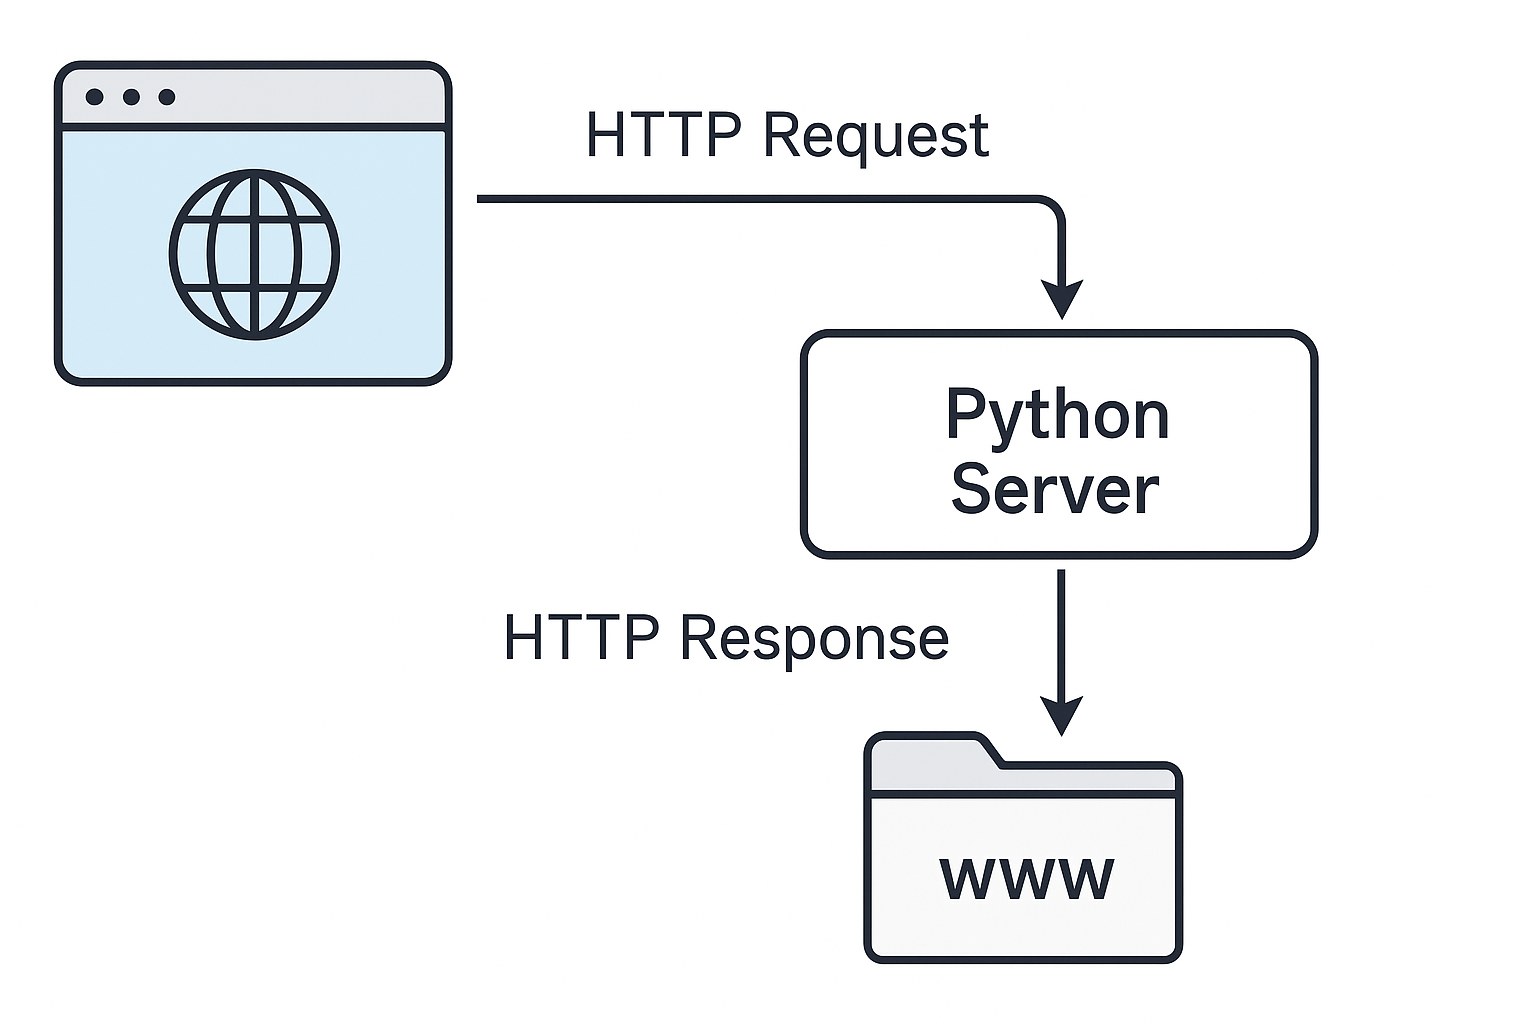
\includegraphics[width=0.5\textwidth]{img/architettura.png}
    \caption{Schema dell'architettura client-server}
    \label{fig:architettura}
\end{figure}

In \Cref{fig:architettura} viene rappresenta l'interazione tra browser, server e file system. Quando un client
invia una richiesta HTTP, il server interpreta la richiesta, individua il file richiesto nella directory \texttt{www/}
e restituisce il contenuto.

\chapter{Implementazione del web server}


\chapter{Sito web statico}

\chapter{Test e risultati}

\chapter{Conclusioni}

\chapter{Appendice}

\end{document}
